
In questo capitolo vengono illustrati tutti i test che sono stati svolti per valutare le performance del sistema CAMUS ...

\section{Sistema di test e modello di simulazione}

\textcolor{red}{Prendere workload model dall'articolo\	
	Definizione di service time e response time\
	spiegare quali test verranno eseguiti nelle prossime sezioni}



Per effettuare i test di workload abbiamo scelto di utilizzare un sistema con coda  M/G/1 \cite{sundarapandian2009probability}. Infatti il nostro sistema si può descrivere con le seguenti caratteristiche:

\begin{itemize}
	\item M/*/*: %a service node where request arrival follows a \emph{markoviano}
	%process, i.e. requests arrive continuously and independently at a
	%constant average rate $\lambda$. We will use this assumption in the
	%characterization of the response time.
	
	\item */G/*: %the service rate distribution is not yet known, so we assume it being a
	%general distribution with fixed mean and variance.
	
	\item */*/1: %a single process (Node.js) serves incoming requests.
\end{itemize}

Di seguito sono riportati le caratteristiche tecniche della macchina di test
\begin{center}
	\begin{tabular}{ l l l }
	Parameter && Value \\ \hline
	CPU && Intel Core i5-3550 \\
	Cores && 4 \\
	CPU frequency && 3.30GHz \\
	RAM && 8 GB DDR3 \\
	Disk && SSD 60 GB + HDD 1TB \\
	Host OS && Microsoft Windows 10 Pro (su SSD)\\
	VM software && Oracle VirtualBox 5.0 \\
	Guest OS && Ubuntu 14.04 (su HDD)
	\end{tabular}
\end{center}

\section{Tempo di risposta ad una singola richiesta}

\textcolor{red}{specificare che i test vengono fatti con 1 core e 1 GB RAM\\
	metodologia di test (uno dietro l'altro)\\
	grafico service time distribution + ricavo lambda saturazione\\
	grafico service time overview + spiegazione di come sono state prese le variabili e risultati\\
	grafico component time + spiegazione}

\section{Tempo di risposta per richieste multiple}

\textcolor{red}{Spiegare metodologia di test (+ riferimenti distribuzioni e perchè è stata scelta)\\
	mostrare 1 core e 1 GB RAM che diventa instabile come predetto prima\\
	spiegare perchè è stato fatto test di scaling e miglioramenti ottenuti e perchè (redis e node sono single threaded)}

\section{Tempo di risposta con condizioni di rete diverse}

Oltre ai test sul carico del server sono stati effettuate delle valutazioni per quanto riguarda le diverse condizioni di utilizzo dell'applicazione mobile. Avendo scelto come caso di studio quello del turismo è sorto spontaneo chiedersi in che modo l'applicazione reagisse in movimento e in diverse condizioni di rete. Per esempio se l'utente si trova a casa propria sotto rete WiFi la velocità di caricamento dei risultati sarà diversa da quella misurata mentre si trova in alta montagna, dove la copertura di rete è spesso minima. Per valutare se comunque i tempi di attesa fossero stati accettabili si è scelto di utilizzare il simulatore iOS e uno strumento aggiuntivo che introduce un ritardo nel caricamento dei dati a seconda delle diverse condizioni di rete specificate. A partire da questo si sono scelte le tre condizioni di rete più significative: WiFi, 3G ed Edge.
All'interno dell'applicazione è stato utilizzato un metodo di test che effettua un numero significativo di richieste verso il server. Il test è stato effettuato utilizzando 50 richieste una successiva alle altre, in modo da non peggiorare il tempo di risposta caricando eccessivamente il server. La query utilizzata è quella di tipo ristoranti, continuamente ripetute. \\
Nella tabella seguente sono mostrati i parametri delle condizioni di simulazione, dove l'Adsl indica la connessione internet utilizzata dal computer e gli altri parametri sono quelli utilizzati nello strumento di modifica delle condizioni di rete:
\begin{center}
	\begin{tabular}{ l l l l l  l l}
		Connection Type && Download Speed  && Upload Speed && Total Delay \\ \hline
		Adsl && 7 Mb/s && 340 Kb/s &&\\ \hline
		Edge && 240 Kb/s && 200 Kb/s && 840 ms \\ 
		3G  && 780 Kb/s && 330 Kb/s && 200 ms \\
		WiFi  && 40 Mb/s && 33 Mb/s && 2 ms \\
	\end{tabular}
\end{center}

Nella Figura \ref{fig:network-time-analysis} sono mostrati i risultati medi per ogni condizione di rete. Come ci si poteva aspettare i tempi di risposta più bassi sono dati dalla connessione WiFi, seguiti dal 3G e successivamente dalla Edge. La differenza tra WiFi e 3G è molto meno marcata, soprattutto perché per provare il tempo risposta è stata utilizzata una connessione a monte non molto performante, mentre per quanto riguarda la connessione Edge c'è molta più differenza, come del resto era prevedibile dalle condizioni di simulazione. In qualunque caso, con l'utilizzo della paginazione con un caricamento scaglionato dei dati e le dimensioni ridotte dei dati, anche i tempi di risposta in condizioni sfavorevoli non sono così alti, consentendo all'utente in qualsiasi caso una soddisfacente esperienza d'uso.

\begin{figure}[ht]
	\centering
	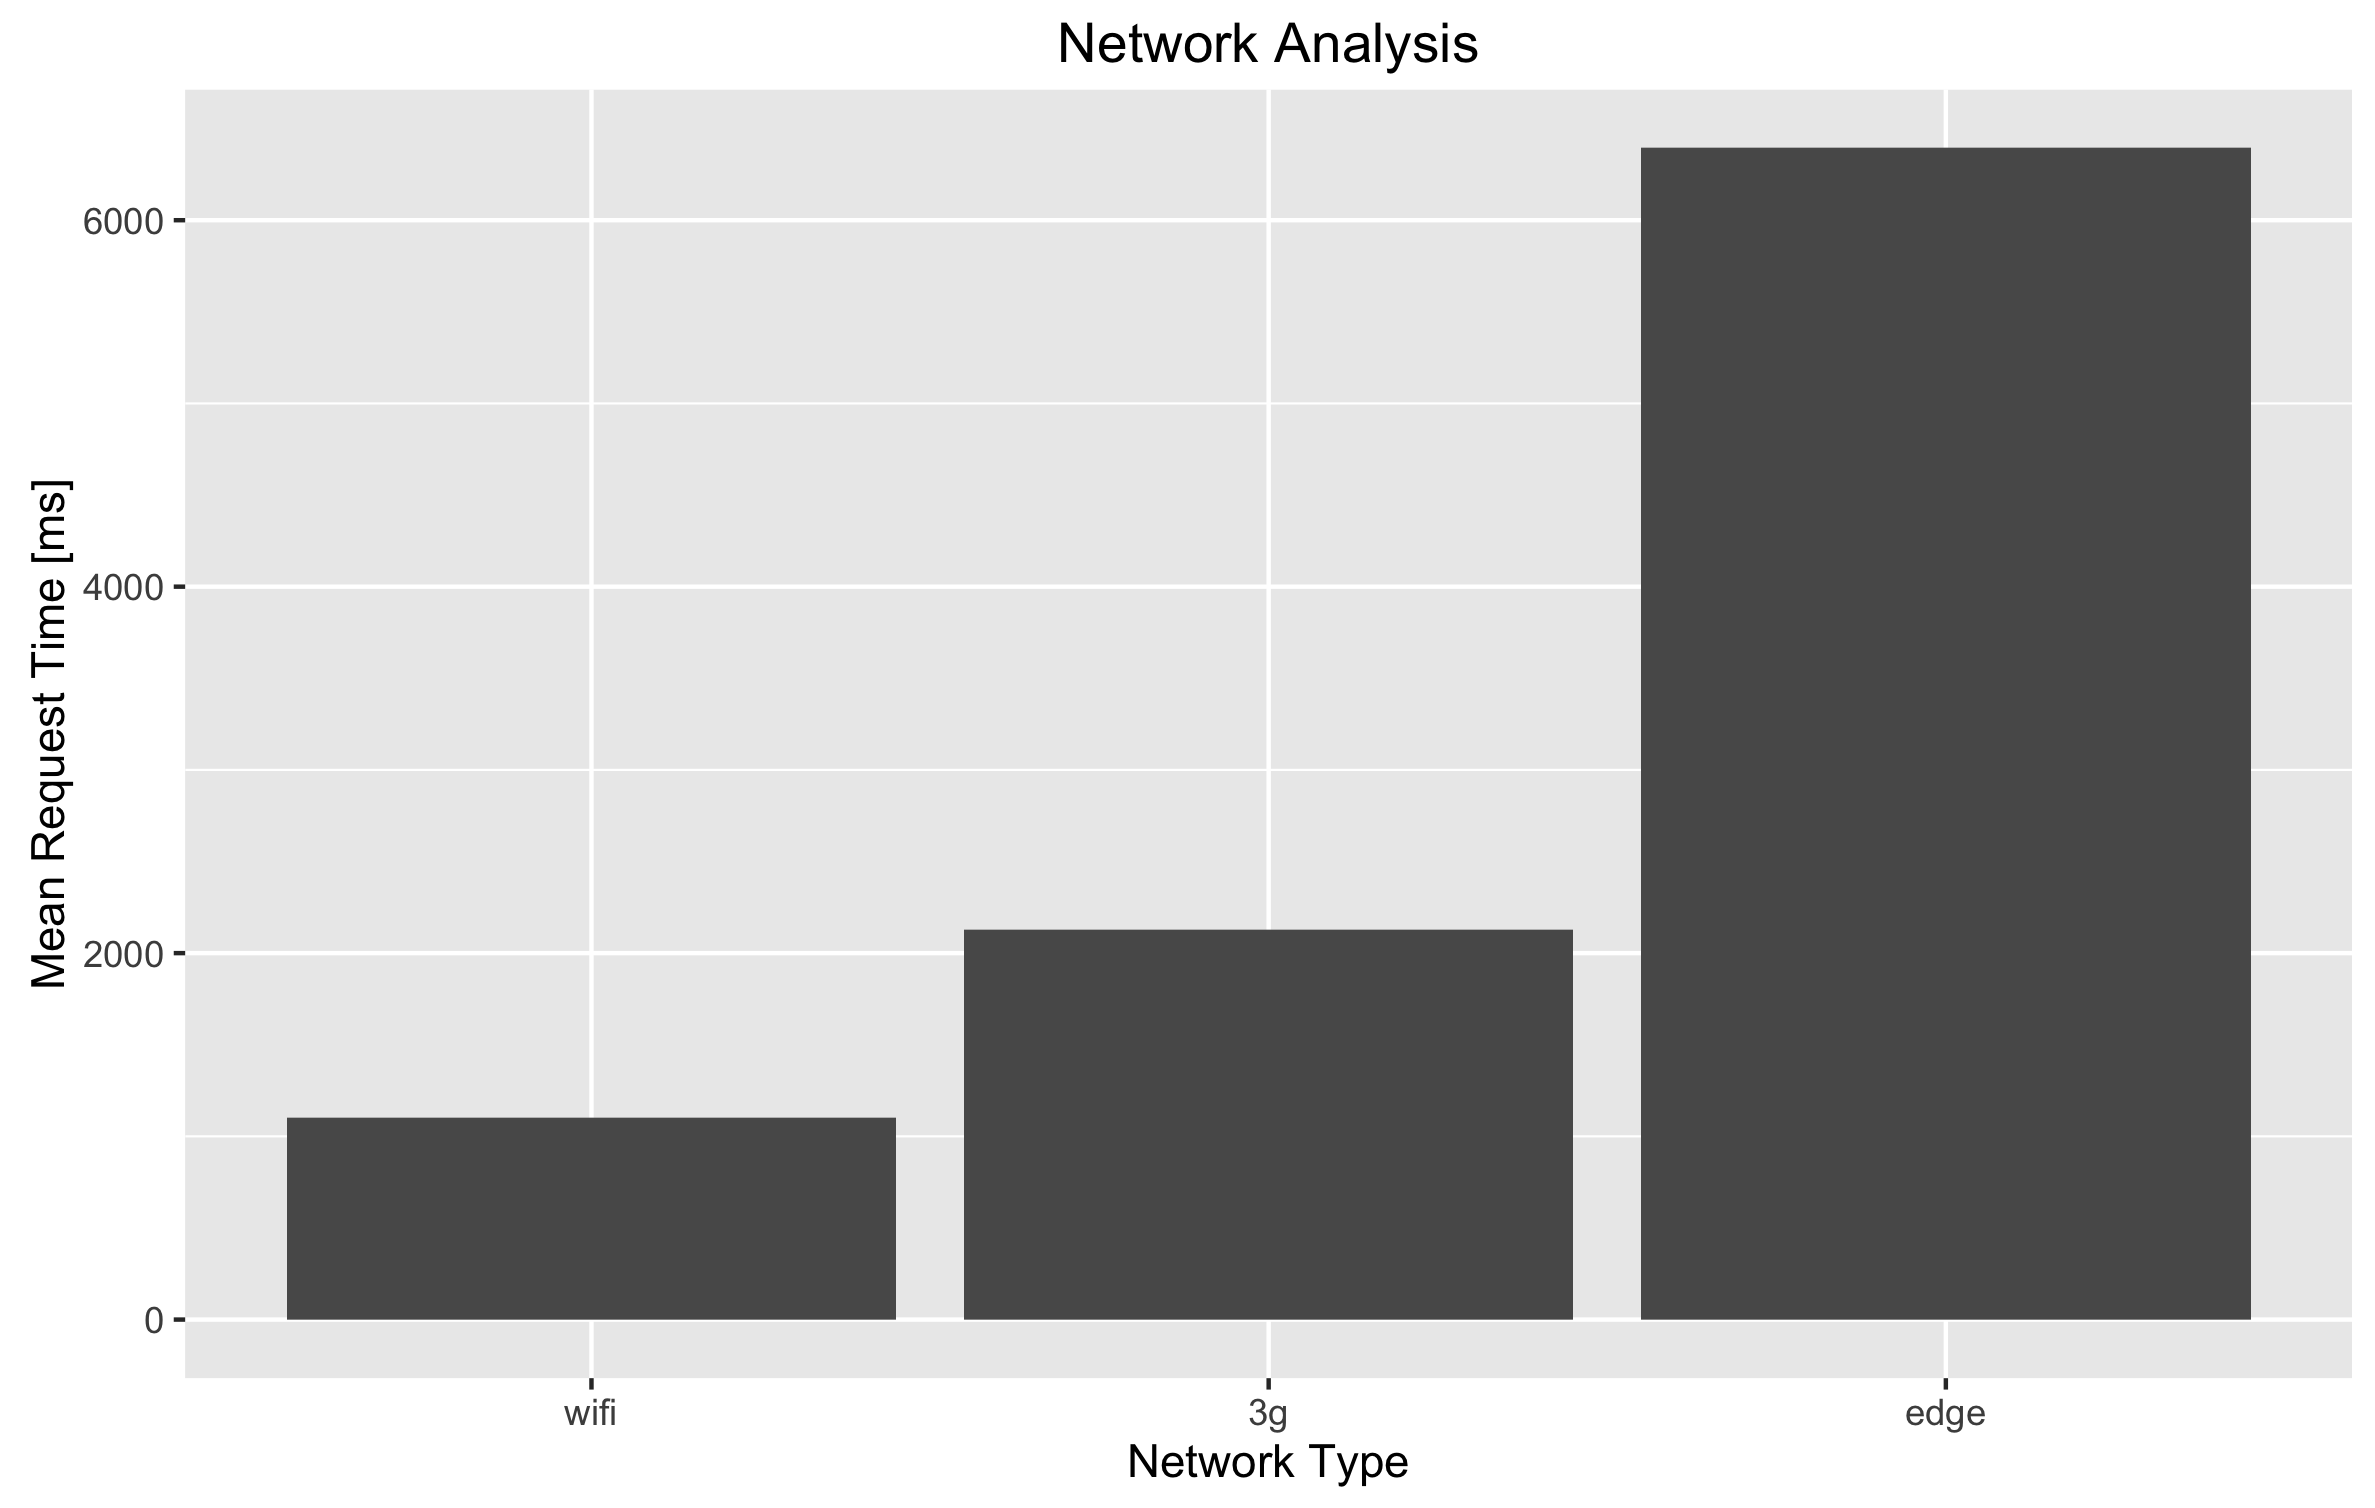
\includegraphics[width=\textwidth]{7-performance/Immagini/network_time_analysis.png}
	\caption{Analisi dei tempi di risposta con reti diverse}\label{fig:network-time-analysis}
\end{figure}